%Suggested order of slides:

%1 slides-51-bpe
%2 slides-52-encoder
%3 slides-53-decoder
%4 slides-54-use-mt
%5 slides-55-trafo-xl

%slides-basics-notation is just a glossary, superseded by cheatsheet.

\subsection{BytePair encoding}
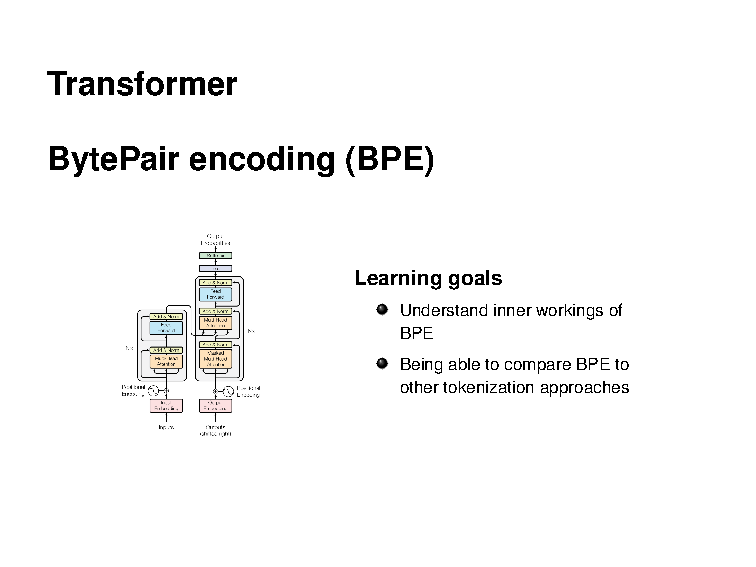
\includepdf[pages=-]{../slides-pdf/slides-51-bpe.pdf}

\subsection{The Encoder}
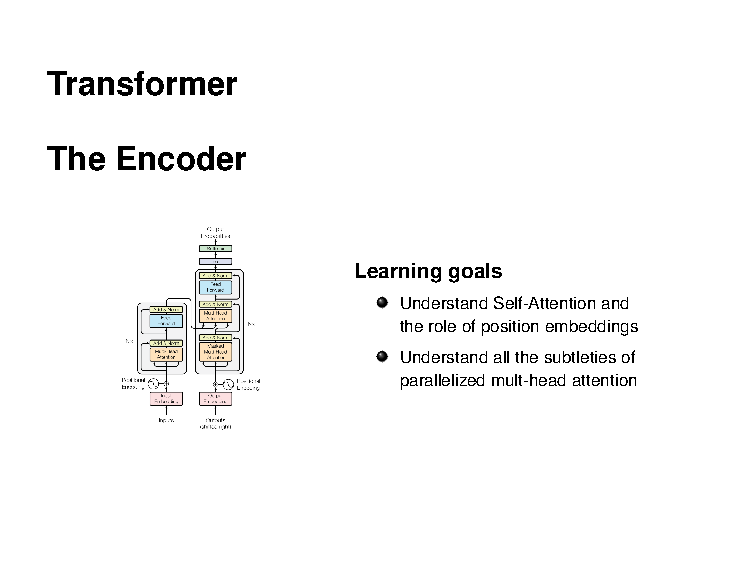
\includepdf[pages=-]{../slides-pdf/slides-52-encoder.pdf}

\subsection{The Decoder}
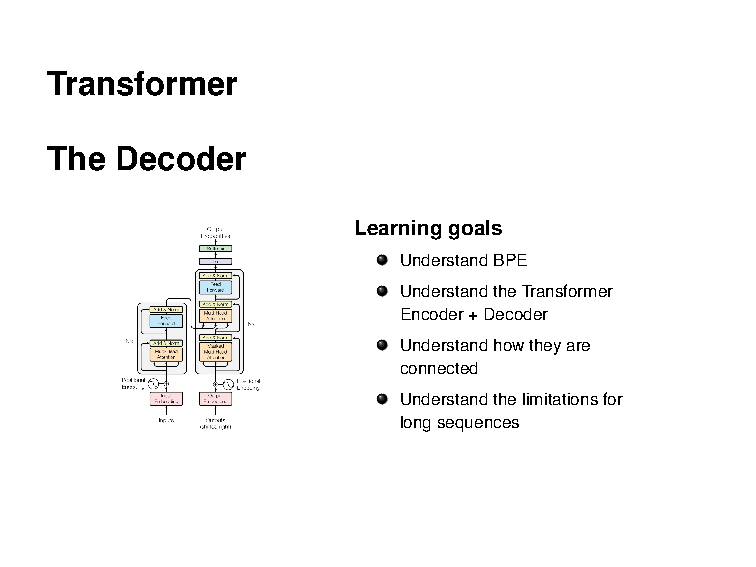
\includepdf[pages=-]{../slides-pdf/slides-53-decoder.pdf}

\subsection{Transformer for MT}
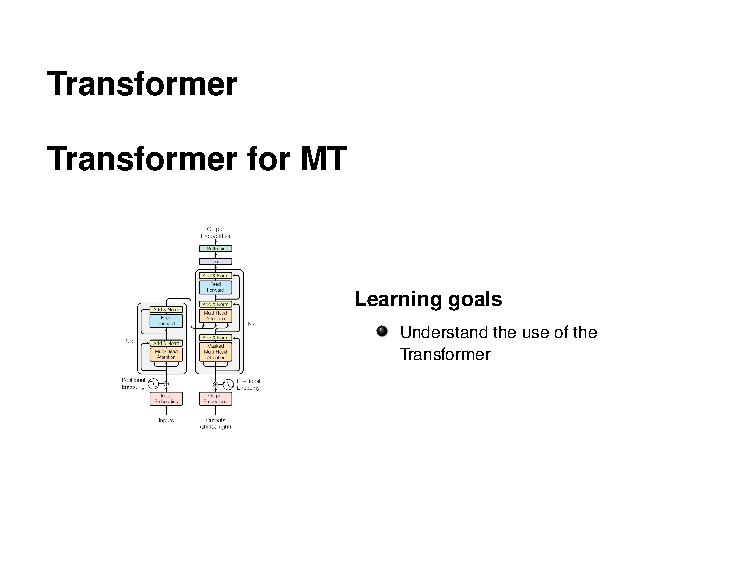
\includepdf[pages=-]{../slides-pdf/slides-54-use-mt.pdf}

\subsection{Transformer XL}
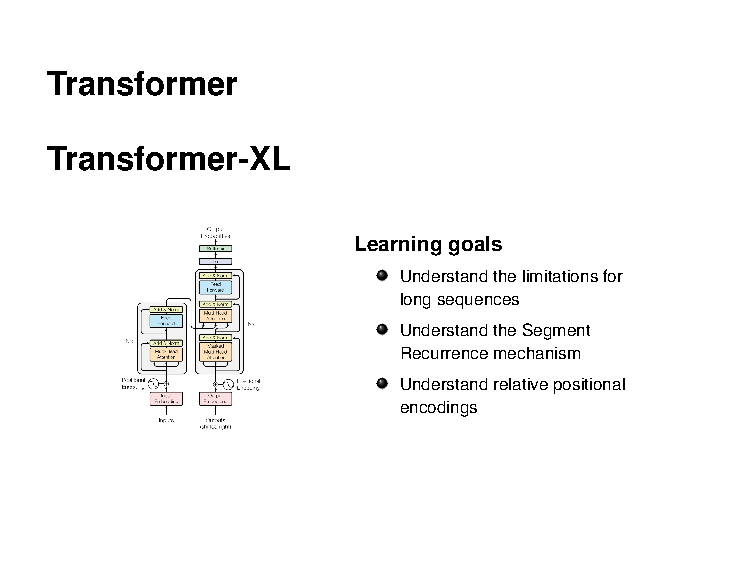
\includepdf[pages=-]{../slides-pdf/slides-55-trafo-xl.pdf}

